\section{Descriptive Statistics}
\subsection{Data reading}
\tab We'll use R's read.csv function to import our data. Our focus will be on the following columns: Memory, Resolution, Manufacturer, Core Speed, Memory Bus, Memory Speed, Process, Pixel Rate, Texture Rate, TMUs, Shader, Memory Bandwidth. This emphasis is crucial since our primary goal is to predict Memory Speed.  We'll check each column for missing values, as minimizing these is essential for accurate prediction.:
\begin{center}
    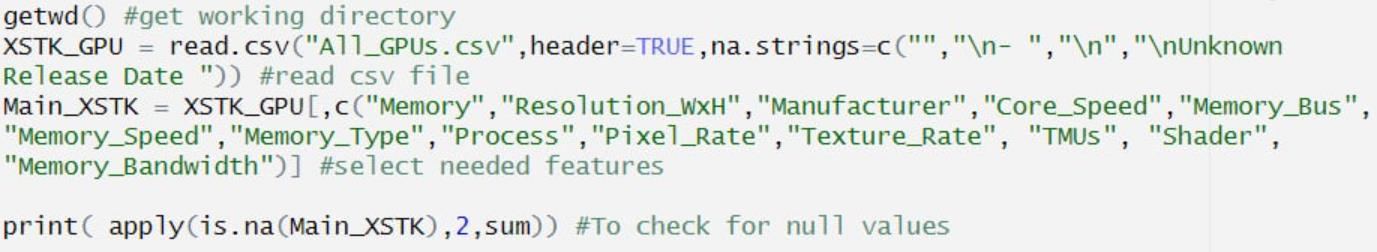
\includegraphics[width=0.8\textwidth]{Read_Data.png}
\end{center}
\tab Then we check for the missing values in the dataset
\begin{center}
    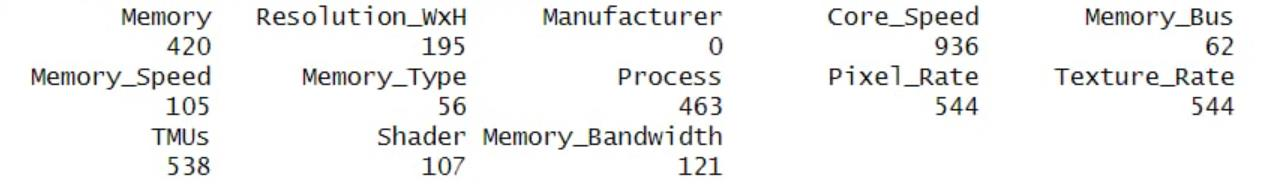
\includegraphics[width=0.8\textwidth]{Checknull.png}
\end{center}
\subsection{Data cleaning}
\tab The missing values comprise less than 30\% of our dataset. Therefore, we'll convert relevant columns to numeric data types and replace N/A values with their corresponding median values to prepare the data for analysis
\begin{center}
    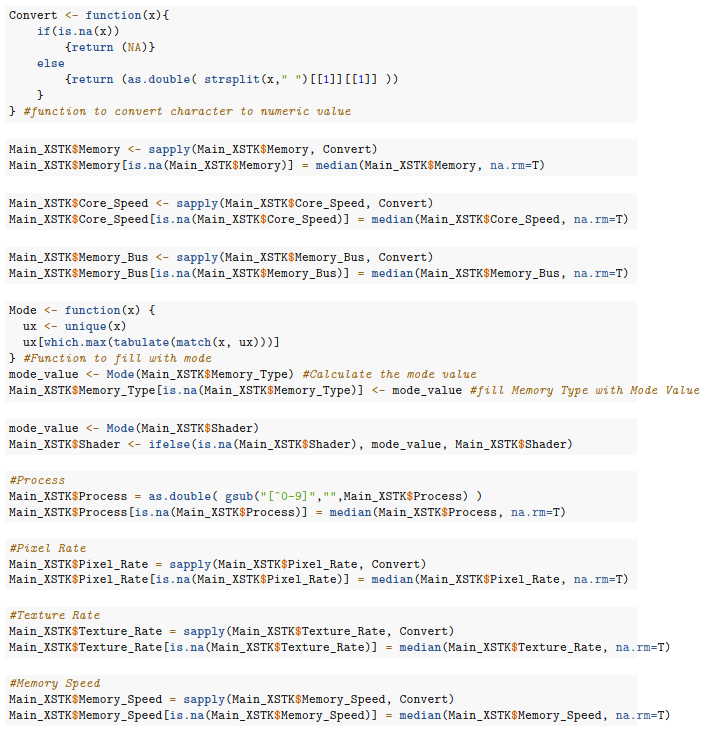
\includegraphics[width=0.8\textwidth]{cleaning.png}
\end{center}

\tab And for some value, we'll use the mode (the most frequent value) to fill in some missing data. This approach helps us preserve the overall shape of the data distribution, especially when dealing with categories
\begin{center}
    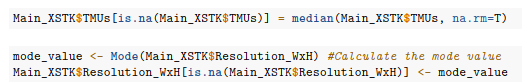
\includegraphics[width=0.8\textwidth]{clean2.png}
\end{center}

\tab After cleaning the data set, we re-check the missing value of the data set again
\begin{center}
    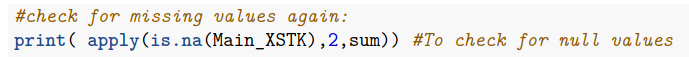
\includegraphics[width=0.8\textwidth]{check.png}
\end{center}
\begin{center}
    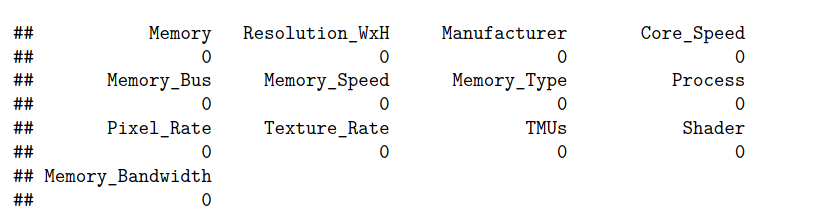
\includegraphics[width=0.8\textwidth]{checked.png}
\end{center}

\tab After checked, There's no missing value in our data set

\subsection{Data visualization}
\subsubsection{Summary table}
\tab We summary all the columns in the data set using "describe"
\begin{center}
    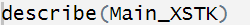
\includegraphics[width=0.8\textwidth]{des.png}
\end{center}
\begin{center}
    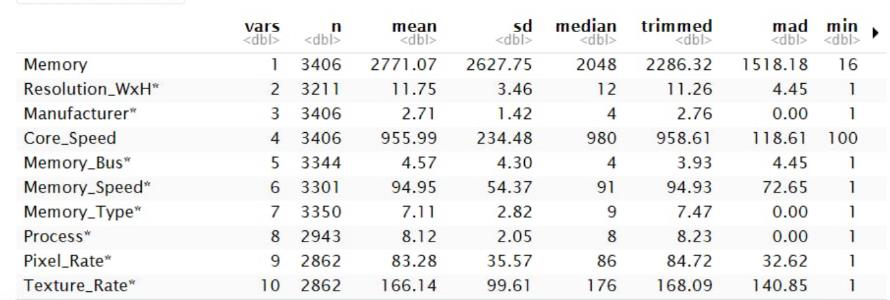
\includegraphics[width=0.8\textwidth]{des1.png}
\end{center}

\subsubsection{Histogram}
\tab Use histograms to analyze the distributions of these 12 key variables: Memory Speed, Memory, Memory Bus, Core Speed, Process, Pixel Rate, Texture Rate, Memory Bandwidth, TMUs, Shader, Resolution WxH, Manufacturer, and Memory Type. This will help us understand their spread, central tendencies, and any potential outliers

\begin{center}
    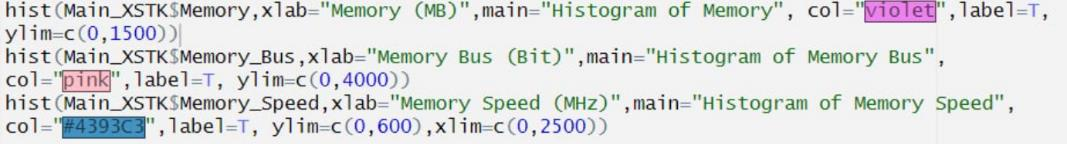
\includegraphics[width=0.7\textwidth]{sk.png}
\end{center}
\begin{center}
    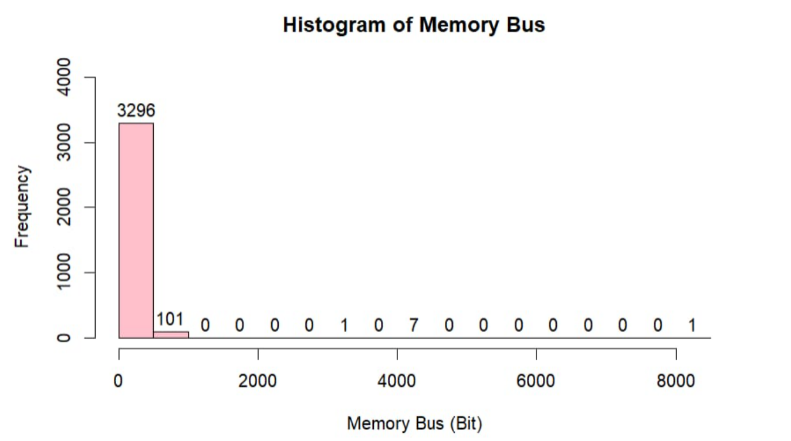
\includegraphics[width=0.7\textwidth]{membush.png}
\end{center}
\begin{center}
    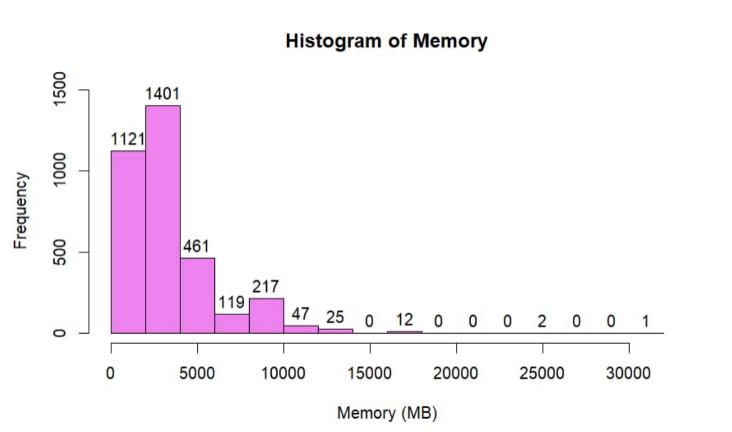
\includegraphics[width=0.7\textwidth]{memh.png}
\end{center}
\begin{center}
    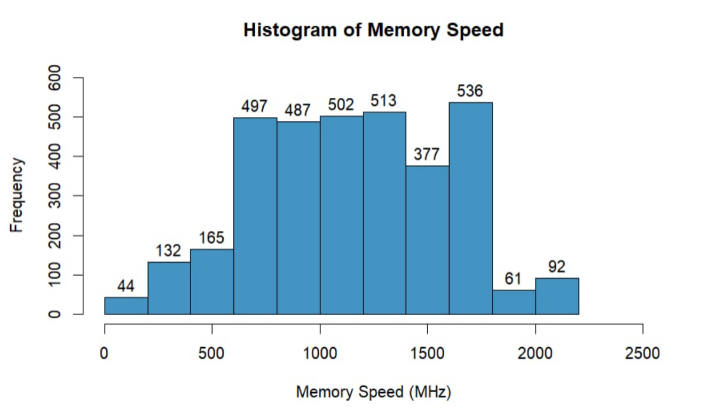
\includegraphics[width=0.7\textwidth]{memspeed.png}
\end{center}

\textbf{Description:}
\begin{itemize}
    \item Histogram of Memory Speed
    \begin{itemize}
        \item The highest frequency is 536 occurs approximately between 1643 and 1786 MHz
        \item The lowest frequency is 44 occurs approximately between 0 and 200 MHz.
        \item This histogram tends to be central.
    \end{itemize}

    \item Histogram of Memory
    \begin{itemize}
        \item The highest frequency is 1401 occurs approximately between 2000 and 4000 MB
        \item The lowest frequency is 0 occurs approximately between 14000 and 16000 MB, from 18000 to 24000 MB, and from 26000 to 30000 MB
        \item This histogram tends to skew left.
    \end{itemize}
    \item Histogram of Memory Bus
    \begin{itemize}
        \item The highest frequency is 3296 occurs approximately between 0 and 5000 Bit.
        \item The lowest frequency is 0 occurs approximately between 1000 and 8000 Bit except from 3000 to 3500 Bit, from 4000 to 4500 Bit and from 8000 to 8500 Bit.
        \item This histogram tends to skew left.
    \end{itemize}
    
\end{itemize}
\textbf{Our next analysis will center on Core Speed, Process, and Pixel Rate.}
\begin{center}
    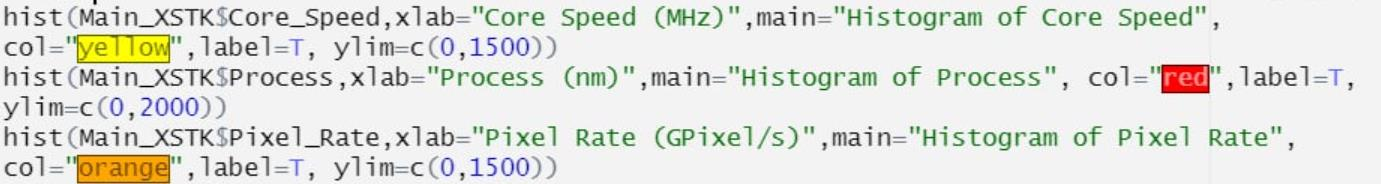
\includegraphics[width=0.7\textwidth]{sk1.png}
\end{center}
\begin{center}
    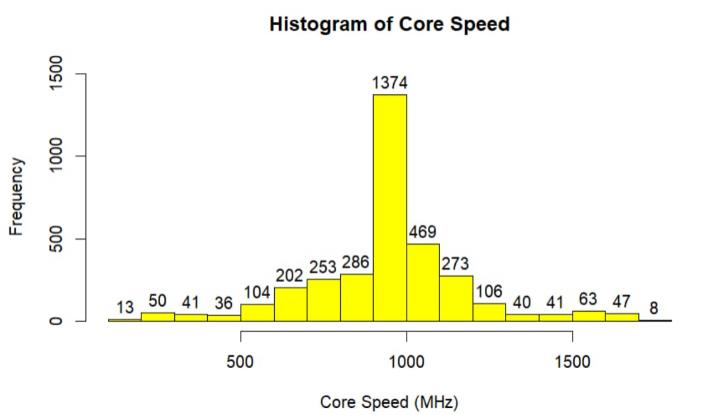
\includegraphics[width=0.7\textwidth]{CSpeed.png}
\end{center}
\begin{center}
    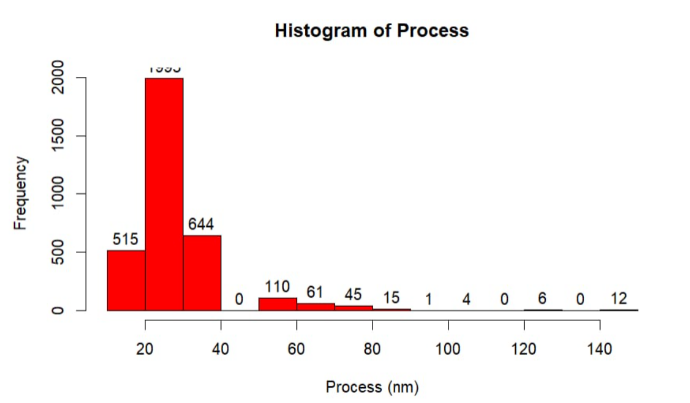
\includegraphics[width=0.7\textwidth]{Process.png}
\end{center}
\begin{center}
    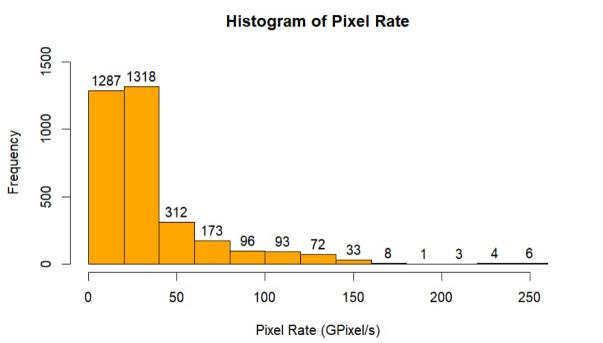
\includegraphics[width=0.7\textwidth]{PixelRatepng.png}
\end{center}

\textbf{Description:}
\begin{itemize}
    \item Histogram of Core Speed
    \begin{itemize}
        \item The highest frequency is 1374 occurs approximately between 900 and 1000 MHz.
        \item The lowest frequency is 8 occurs approximately between 1700 and 1800 MHz.
        \item This histogram tends to be central.
    \end{itemize}

    \item Histogram of Process
    \begin{itemize}
        \item The highest frequency is 1993 occurs approximately between 20 and 30nm.
        \item The lowest frequency is 0 occurs approximately between 40 and 50 MB, from 110 to 120 nm, and from 130 to 140 nm.
        \item This histogram tends to skew left.
    \end{itemize}
    \item Histogram of Pixel Rate
    \begin{itemize}
        \item The highest frequency is 1318 occurs approximately between 20 and 40 GPixel/s.
        \item The lowest frequency is 1 occurs approximately between 180 and 200.
        \item This histogram tends to skew left.
    \end{itemize}
\end{itemize}

\textbf{Now, let's shift our attention to Texture Rate, Memory Bandwith, and TMUs and explore their characteristics.}

\begin{center}
    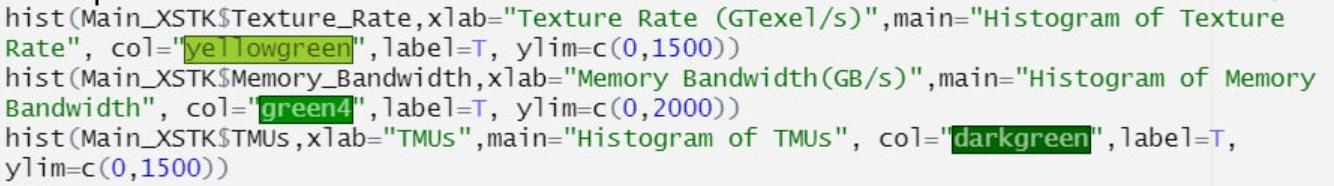
\includegraphics[width=0.7\textwidth]{sk2.png}
\end{center}
\begin{center}
    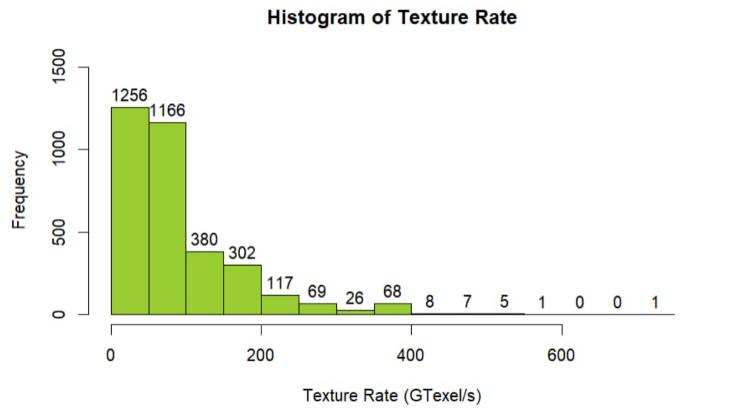
\includegraphics[width=0.7\textwidth]{text.png}
\end{center}
\begin{center}
    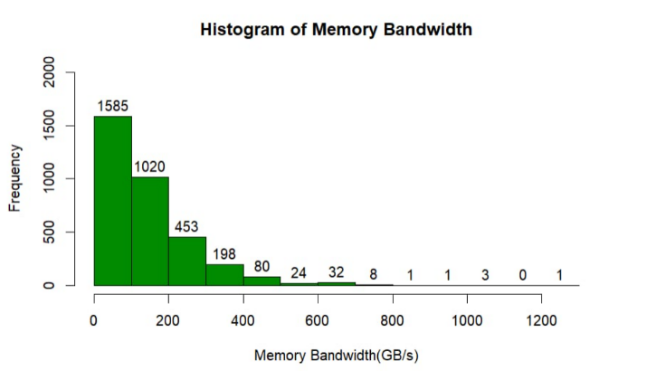
\includegraphics[width=0.7\textwidth]{bandwidth.png}
\end{center}
\begin{center}
    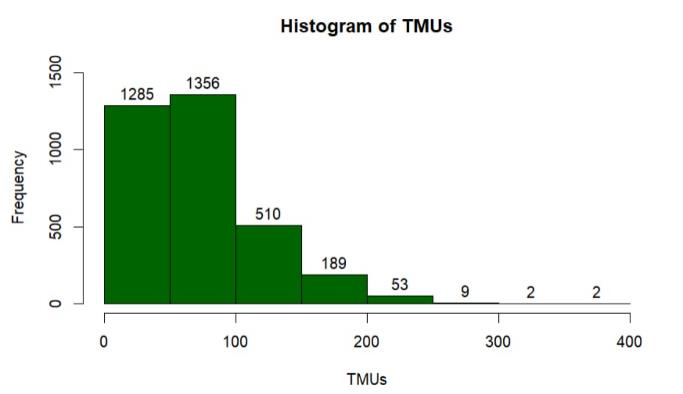
\includegraphics[width=0.7\textwidth]{TMUs.png}
\end{center}


\textbf{Description:}
\begin{itemize}
    \item Histogram of Texture Rate
    \begin{itemize}
        \item The highest frequency is 1256 occurs approximately between 0 and 50 GTexel/s.
        \item The lowest frequency is 0 occurs approximately between 600 and 700 GTexel/s.
        \item This histogram tends to skew left.
    \end{itemize}

    \item Histogram of Memory Bandwidth
    \begin{itemize}
        \item The highest frequency is 1585 occurs approximately between 0 and 100 GB/s.
        \item The lowest frequency is 0 occurs approximately between 1100 and 1200 GB/s.
        \item  This histogram tends to skew left.
    \end{itemize}
    \item Histogram of TMUs
    \begin{itemize}
        \item The highest frequency is 1356 occurs approximately between 50 and 100.
        \item The lowest frequency is 2 occurs approximately between 300 to 400.
        \item This histogram tends to skew left.
    \end{itemize}
\end{itemize}
\textbf{Next, we will analyze Shader, Resolution} 
\begin{center}
    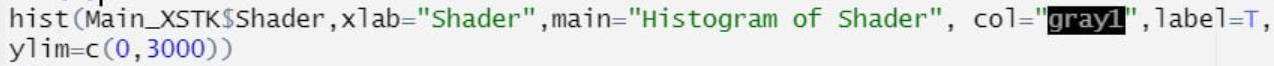
\includegraphics[width=0.7\textwidth]{shader.png}
\end{center}
\begin{center}
    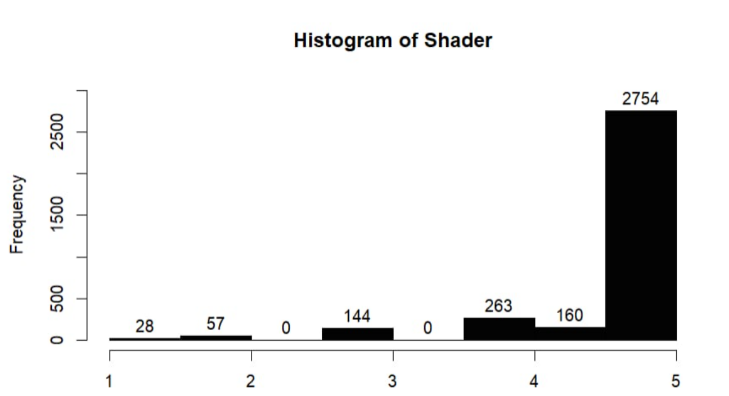
\includegraphics[width=0.7\textwidth]{shader1.png}
\end{center}
\begin{center}
    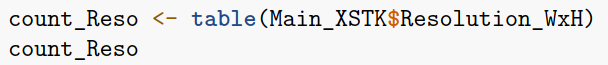
\includegraphics[width=0.7\textwidth]{res.png}
\end{center}
\begin{center}
    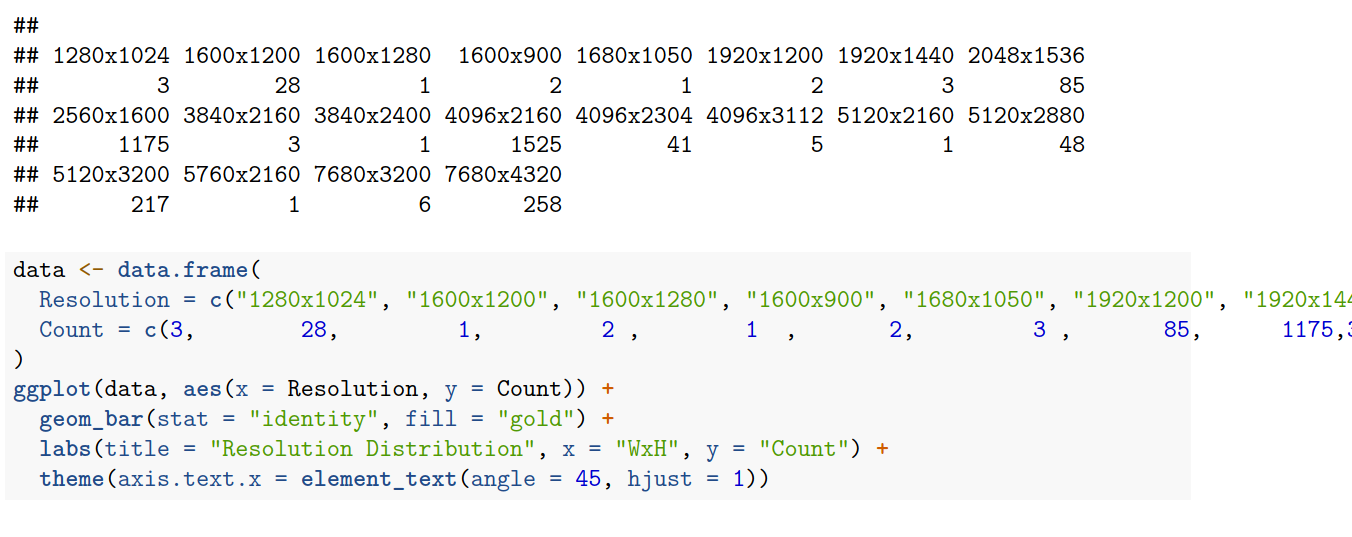
\includegraphics[width=0.7\textwidth]{res1.png}
\end{center}
\begin{center}
    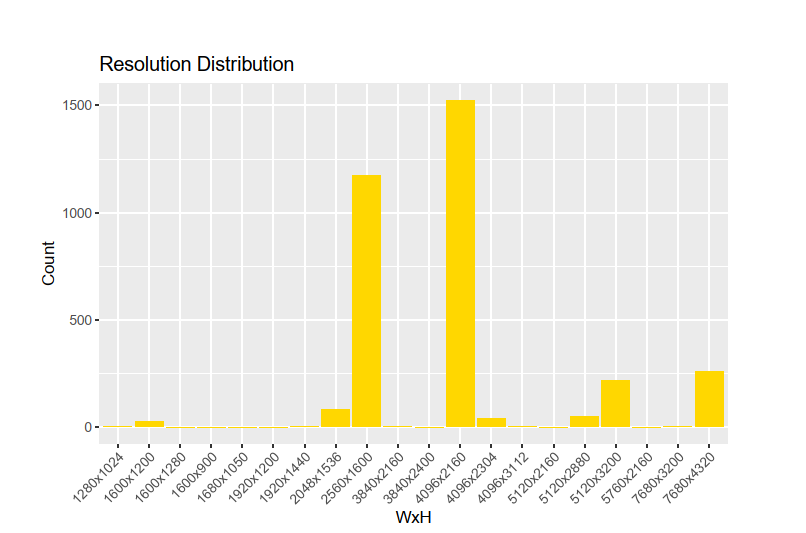
\includegraphics[width=0.7\textwidth]{res2.png}
\end{center}

\textbf{Description:}
\begin{itemize}
    \item Histogram of Shader
    \begin{itemize}
        \item The highest frequency is 2754 occurs approximately between 4.5 and 5.
        \item The lowest frequency is 0 occurs approximately between 2 and 2.5 and from 3 to 3.5.
        \item This histogram tends to skew right.
    \end{itemize}

    \item Histogram of Resolution
    \begin{itemize}
        \item The highest frequency is 1525 occurs at 4096x2160.
        \item The lowest frequency is 1 occurs at 1600x1200, 1600x1280, 1680x1050, 3840x2400, 5120x2160, and 5760x2160.
        \item  This histogram tends to fluctuate.
    \end{itemize}
\end{itemize}

\textbf{Last, we are going to analyze the Memory Type and Manufacturer}

\begin{center}
    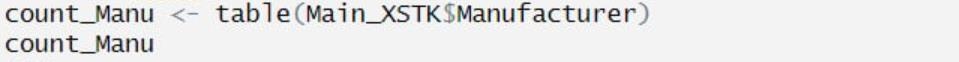
\includegraphics[width=0.7\textwidth]{manu.png}
\end{center}
\begin{center}
    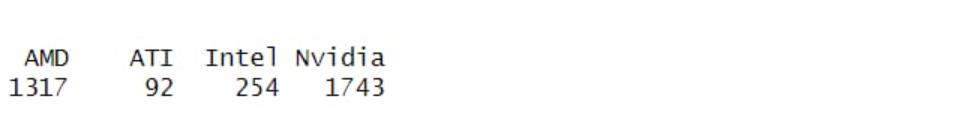
\includegraphics[width=0.7\textwidth]{manu1.png}
\end{center}
\begin{center}
    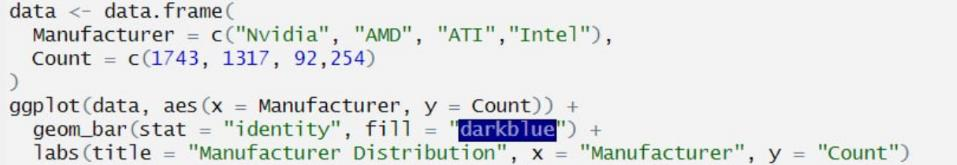
\includegraphics[width=0.7\textwidth]{manu2.png}
\end{center}
\begin{center}
    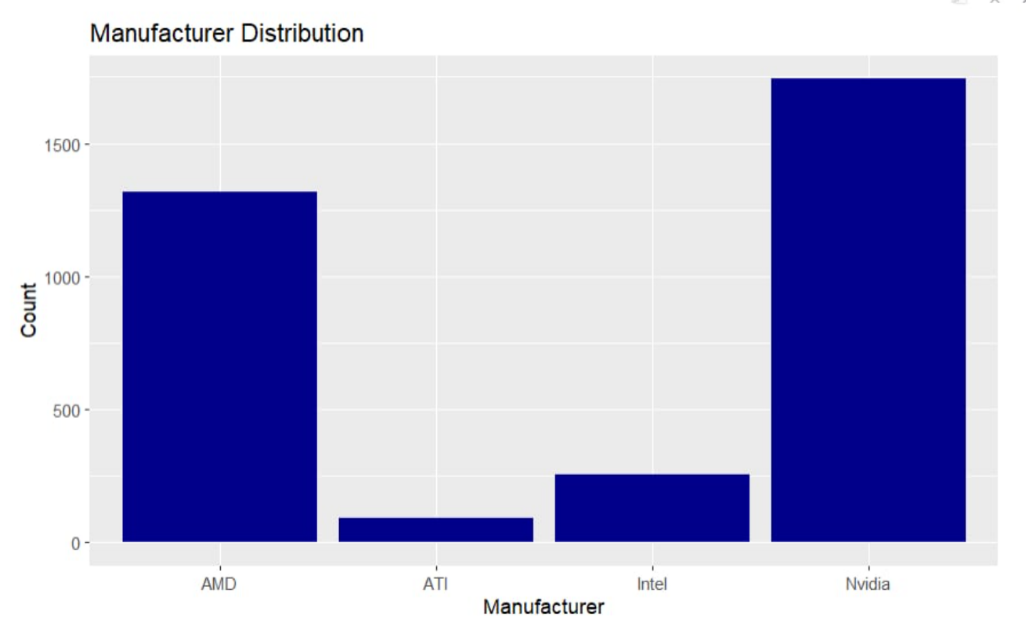
\includegraphics[width=0.7\textwidth]{manu3.png}
\end{center}
\begin{center}
    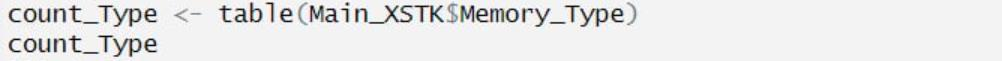
\includegraphics[width=0.7\textwidth]{type1.png}
\end{center}
\begin{center}
    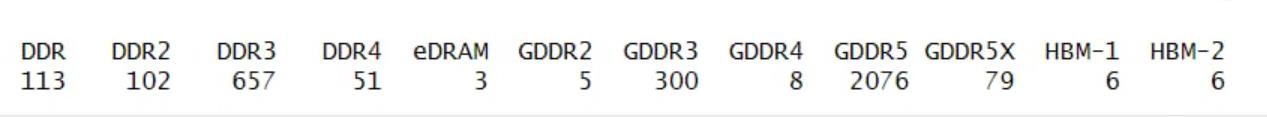
\includegraphics[width=0.7\textwidth]{type2.png}
\end{center}
\begin{center}
    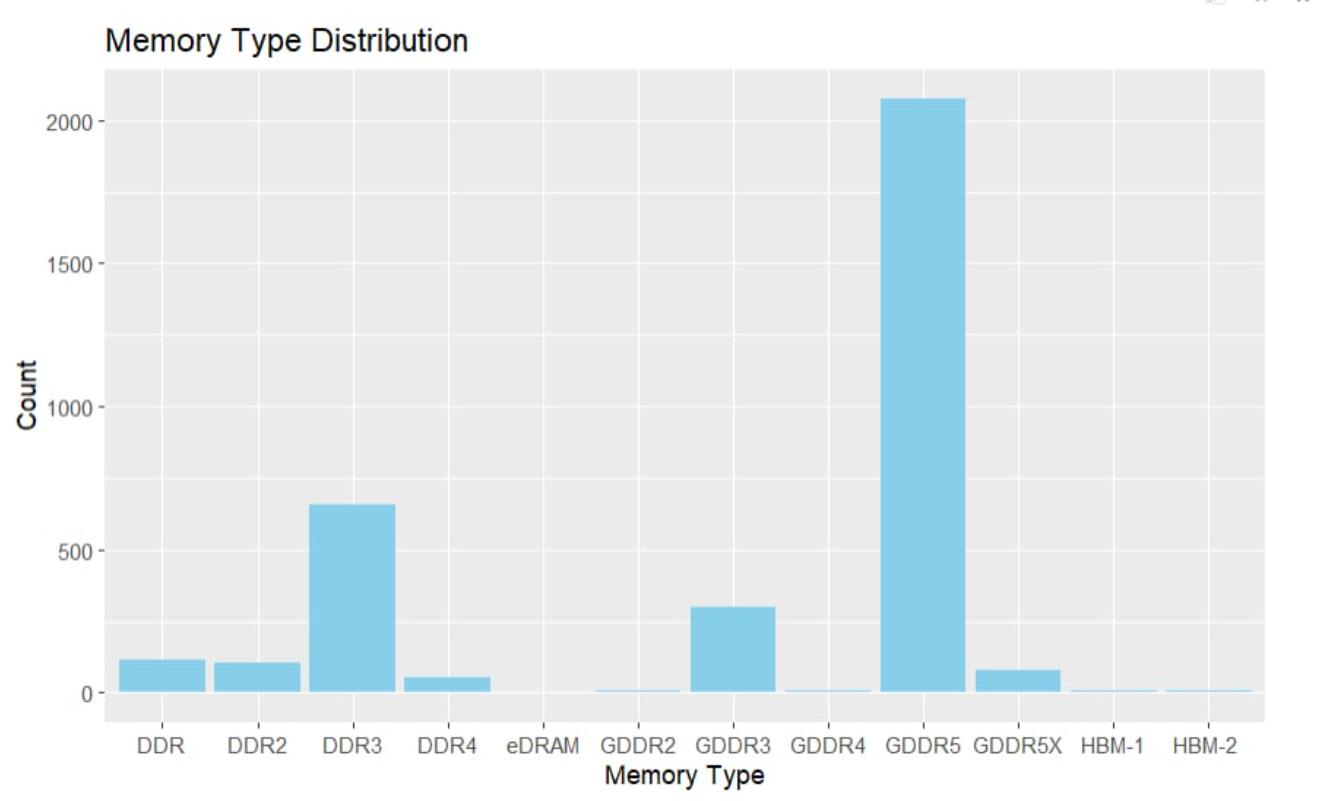
\includegraphics[width=0.7\textwidth]{type3.png}
\end{center}

\textbf{Description:}
\begin{itemize}
    \item Histogram of Memory Type
    \begin{itemize}
        \item The highest frequency is 2754 occurs approximately between 4.5 and 5.
        \item The lowest frequency is 0 occurs approximately between 2 and 2.5 and from 3 to 3.5.
        \item This histogram tends to fluctuate.
    \end{itemize}

    \item Histogram of Manufacturer
    \begin{itemize}
        \item The highest frequency is 1743 occurs at NVIDEA.
        \item The lowest frequency is 92 occurs at ATI., 5120x2160, and 5760x2160.
        \item  This histogram tends to fluctuate.
    \end{itemize}
\end{itemize}

\subsection{Boxplots}
\begin{center}
    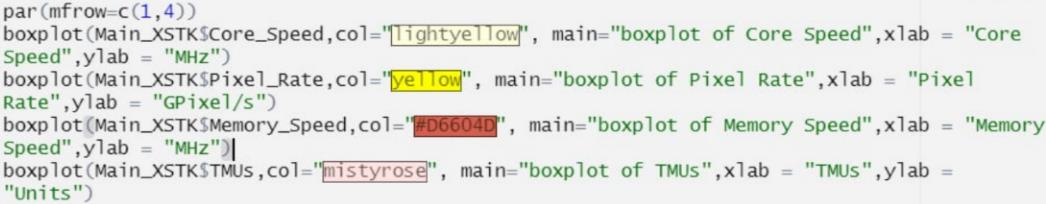
\includegraphics[width=0.7\textwidth]{bp1.png}
\end{center}
\begin{center}
    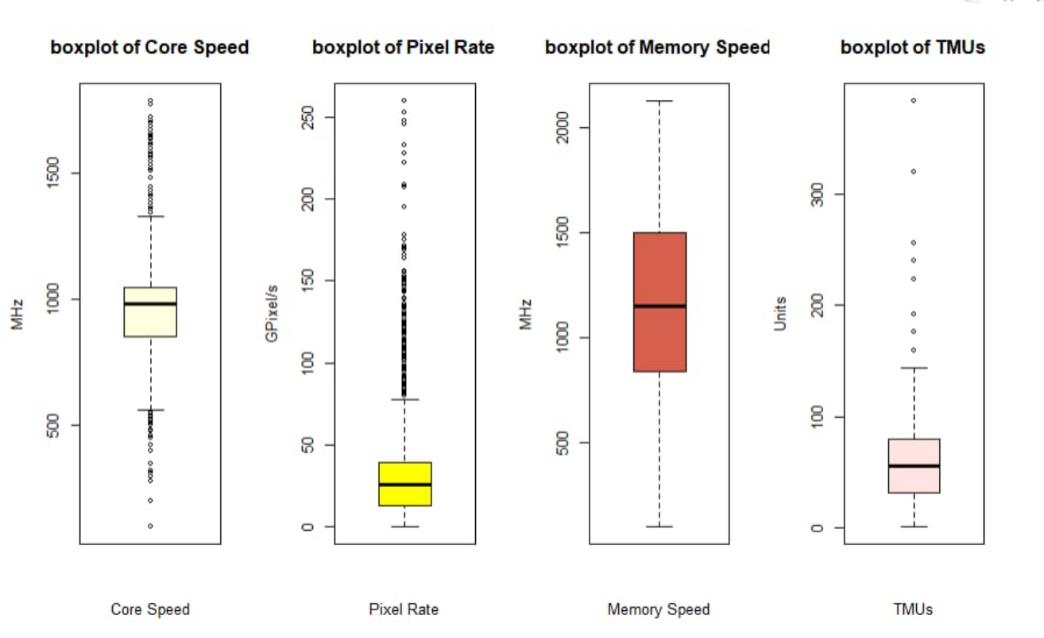
\includegraphics[width=0.7\textwidth]{bp2.png}
\end{center}
\begin{center}
    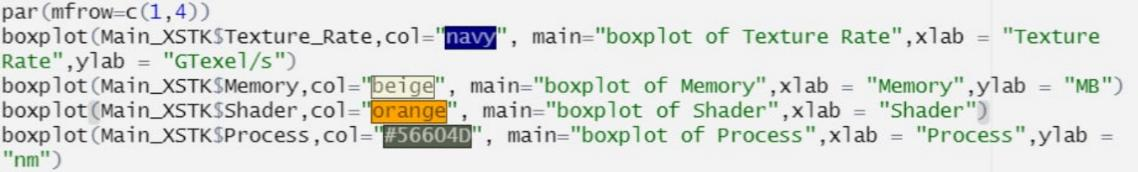
\includegraphics[width=0.7\textwidth]{bp3.png}
\end{center}
\begin{center}
    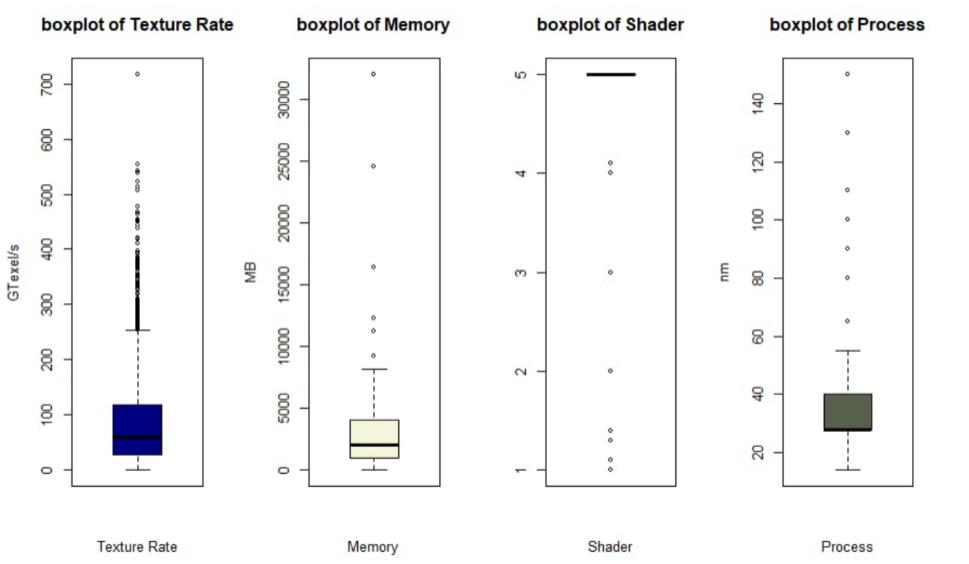
\includegraphics[width=0.7\textwidth]{bp4.png}
\end{center}
\begin{center}
    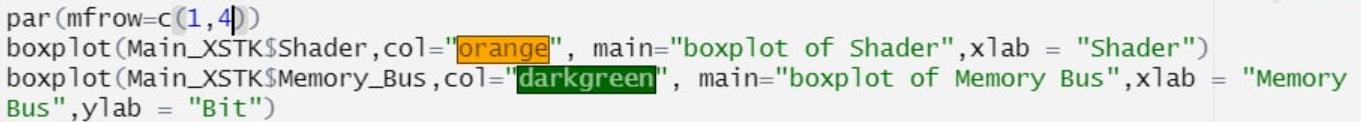
\includegraphics[width=0.7\textwidth]{bp5.png}
\end{center}
\begin{center}
    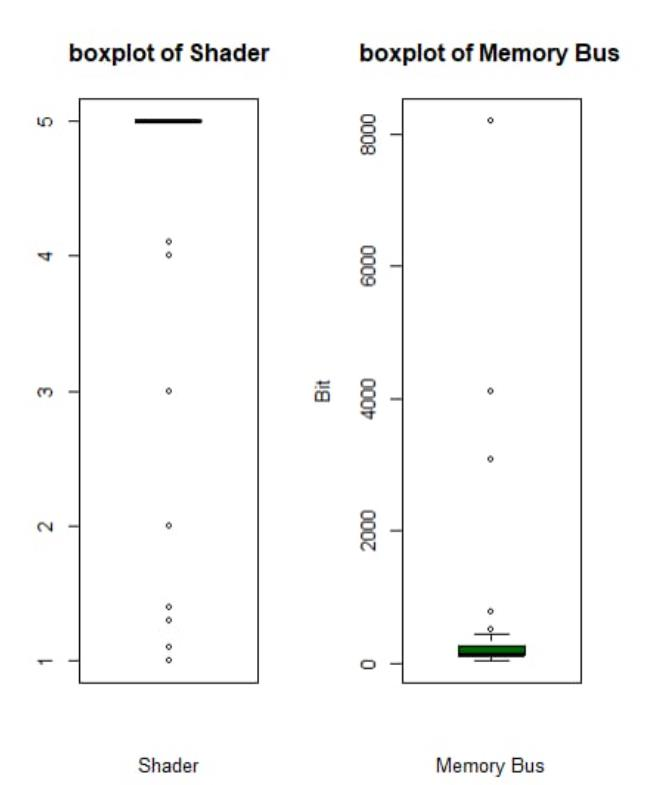
\includegraphics[width=0.7\textwidth]{bp6.png}
\end{center}
\tab \textbf{Comment:} We observe that each output is based on input data that is distributed and exhibits in a similar pattern except for Memory Speed with a wider value range and Shader with tiny range of value. It is not feasible to accurately predict the price by solely considering one variable